\chapter{Problemspezifikation}\label{problemspezifikation}

In diesem Kapitel wird die Selbsteinbettung von Taskgraphen in Mehrprozessorsystemen vorgestellt. Am Beispiel von einem Network-on-Chip (NoC) werden dessen Architektur und ihre Besonderheiten näher betrachtet. Danach wird das Constraint-Satisfaction-Problem (CSP) definiert und die Bedingungen (engl. \textit{Constraints}) für die Architektur festgelegt.

\section{Selbsteinbettung in Mehrprozessorsysteme}
In einem Mehrprozessorsystem \cite{Mehrprozessorsysteme} arbeiten mehrere Zentralprozessoren zusammen. 
Mehrprozessorsysteme erlauben die Verteilung der Aufträge auf mehrere physische Zentralprozessoren und helfen somit den Durchsatz zu erhöhen. Das Betriebssystem verteilt die Anwendungen (engl. \textit{Application}) und deren Teilaufgaben (engl. \textit{Task}) an die Zentralprozessoren.  \\%(Quelle:$http://gd.tuwien.ac.at/study/hrh-glossar/12-1_1.htm$) \\
 


\ \\
Bei der betrachteten Architektur (Abbildung ~\ref{fig:nocbild}) handelt es sich um ein heterogenes Mehrprozessorsystem. Kennzeichnend dafür ist die Verwendung verschiedener Typen von Zentralprozessoren. Diese werden im Weiteren Kacheln genannt. Die einzelnen Kacheln sind in einem Netzwerk -- einem sogenannten Network-on-Chip (NoC) \cite{mappingNocArchitectures} \cite{NOC} -- miteinander verbunden. Das Netzwerk ist zu einem regelmäßigen rechteckigen Gitter von Kacheln geordnet, welches N hoch und M breit ist. Die direktbenachbarten Kacheln sind mit gerichteten Links  $l_i \in L$ (Abbildung ~\ref{fig:links}) in beide Richtungen verbunden. Die Kacheln k $\in$ K sind durch die Koordinaten (x,y) definiert:
%\begin{equation}
% \forall k \in K: k = \{(x, y) | 0 \leq x < N , 0 \leq y < M \}
%\label{kacheln}
%\end{equation}
%\todo{keine einfärbung und sowas}

Eine Kachel kann einen Task ausführen, wenn alle Constraints (Abschnitt \ref{Randbedingungen}) erfüllt sind. Einer dieser Randbedingungen ist der Max-Hop-Constraint. Diese besagt, dass zwei miteinander agierenden Task eine Manhattan-Distanz  $d_m$ (Formel \ref{formel2})nicht überschreiten dürfen. 
%Um zu kennzeichnen, dass eine Kachel einen Task ausführt, wird die Kachel eingefärbt. Es kann aber auch vorkommen, dass eine Kachel während des Betriebs fehlerhaft wird. Diese defekte Kachel sind mit der Farbe rot markiert. Der Abstand zwischen zwei Kacheln $k_1$ und $k_2$ berechnet sich mit Hilfe der Manhattandistanz  $d_m$.
\begin{equation}
d_m (k_1,k_2) = \mid k_1.x - k_2.x \mid + \mid k_1.y - k_2.y \mid 
\label{formel2}
\end{equation}

\begin{figure}[H]\centering
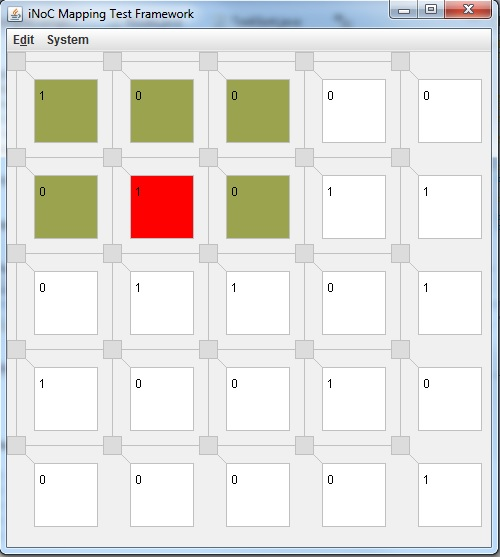
\includegraphics[width = 70mm]{bilder/NoC.jpg}
\caption{Simulation eines heterogenes Network-On-Chip: Die belegten Kacheln sind mit grün und die defekten Kacheln mit rot markiert. In jeder Kachel steht der Ressourcentyp (0 oder 1).}\label{fig:nocbild}
\end{figure}

\begin{figure}[H]\centering
  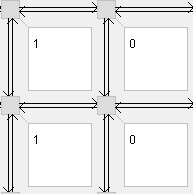
\includegraphics[width = 30mm]{bilder/Links.jpg}
  \caption{Die benachbarten Kacheln sind mit gerichteten Links in beide Richtungen verbunden.}\label{fig:links}
\end{figure}
\ \\
Jede Anwendung, die aus mehreren Teilaufgaben, den sogenannten Tasks, besteht, besitzt einen Taskgraphen (Abbildung ~\ref{fig:taskgraph}). Dieser wird zur Entwurfszeit des Programms erstellt und stellt die Anforderungen, die für eine erfolgreiche Einbettung notwendig sind, graphisch dar.

 %Die konkreten Anforderungen werden im Kapitel \todo{korrekter Verweis} näher dargelegt. \\ \\
%% die\texttt{
%%Einbettung, die für die gewünschten nicht-funktionalen Eigenschaften der Anwendung
%%während der Ausführung nötig sind. Das kann zum Beispiel ein garantierter Datendurchsatz
%%oder eine maximale Latenz sein. Es wird angenommen, dass die Anwendung periodisch
%%ausgeführt wird und regelmäßig Nachrichten zwischen den Tasks versendet. Diese
%%Kommunikation der Tasks untereinander wird mit Kommunikationsknoten dargestellt.
%%Die folgende Definition ist ähnlich zum Anwendungsgraphen in, erlaubt
%%aber, an}ders als dieser, beliebige Kommunikationsstrukturen.
\begin{figure}[H]\centering
  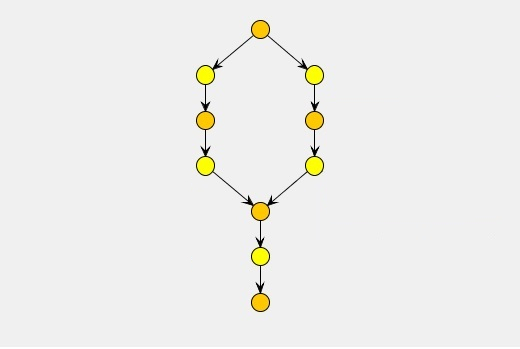
\includegraphics[width = 150mm]{bilder/taskgraph2.jpg}
  \caption{Der Taskgraph besteht aus orangefarbenen Task- und gelbgefärbten Kommunikationsknoten}\label{fig:taskgraph}
\end{figure}
\ \\
Eine Applikation besteht aus miteinander verbundenen Taskknoten $t \in T$ und Kommunikationsknoten $c \in C$. Es sind nur Kanten zwischen diesen beiden Knotentypen erlaubt. Außerdem besitzt jeder Kommunikationsknoten \textbf{genau} eine Eingangskante und eine Ausgangskante. Dem Task- und dem Kommunikationsknoten werden verschiedenartige Bedingungen übergeben, die zu erfüllen sind. Die verschiedenen Typen von Constraints sind je nach Anwendungsgebiet erweiterbar.

\begin{itemize}
\item Taskknoten $t_i\in T$
\begin{itemize}
\item \textit{TypeConstraint}: \\
Der Task benötigt einen bestimmten Kacheltyp
\item \textit{TaskWorkloadConstraint}: \\
Der Task benötigt die Kachel zu einem gewissen Prozentsatz
\item \dots 
\label{Taskknoten}
\end{itemize}
\item Kommunikationsknoten $c_i \in C$:
\begin{itemize}
\item \textit{BandwidthConstraint}: \\
Jeder Link auf der Route zwischen den eingebetteten Tasks muss eine bestimmte Bandbreite für die Kommunikation freihaben.
%\item $c_i$.messageSize: Die Nachrichtengröße
%\item $c_i$.period: Das Intervall, in dem die Nachrichten geschickt werden /todo{Abstand in dem die Nachrichten geschickt werden?}
\item \textit{MaxHopConstraint}: \\
Maximale Manhattan-Distanz zwischen zwei Tasks, die mit einer Kommunikation in Verbindung stehen. 
\item \dots
\label{Kommunikationsknoten}
\end{itemize}
\end{itemize}

%Hier eine Auflistung von möglichen \\ \\
%die Kanten dabei nur zwischen diesen beiden Knotentypen existieren, also nur von Task- zu
%Kommunikationsknoten und umgekehrt. Für die Kommunikationsknoten gilt zudem
%die Einschränkung, dass sie genau eine ein- und ausgehende Kante besitzen müssen. Dadurch
%sind einerseits keine Multicasts möglich und andererseits keine Kommunikation
%ohne einen Zieltask. Ein Task kann beliebig viele ein- und ausgehende Kanten haben.
%\ \\ \\
%Folgende Informationen sind im Taskgraph (Abbildung ~\ref{fig:taskgraph}) für jeden Task- bzw. Kommunikationsknoten einsehbar.
%\begin{itemize}
%\item Taskknoten $t_i\in T$
%\begin{itemize}
%\item $t_i$.ressourceRequirements: Die Anforderungen an die Ressource in Prozent
%\item $t_i$.ressourceType: Den vom Task benötigten Ressourcetypen
%\item $t_i$.ProcessingTime: Die Laufzeit des Tasks
%\label{Taskknoten}
%\end{itemize}
%\item Kommunikationsknoten $c_i \in C$:
%\begin{itemize}
%\item $c_i$.bandwidth: Die Datenübertragungsrate der Nachricht
%%\item $c_i$.messageSize: Die Nachrichtengröße
%%\item $c_i$.period: Das Intervall, in dem die Nachrichten geschickt werden /todo{Abstand in dem die Nachrichten geschickt werden?}
%\item $c_i$.hopLimit: Maximale Manhattan-Distanz (Formel ~\ref{formel2}) zwischen sendendem und empfangendem Taskknoten
%\label{Kommunikationsknoten}
%\end{itemize}
%\end{itemize}
\ \\
Das Ziel des Algorithmus ist es, für jeden Task eine Kachel zu finden, so dass alle Anforderungen des Taskgraphen erfüllt sind. Ist dies nicht möglich, soll der Algorithmus sich beenden und einen Fehlschlag der Einbettung melden. Im Abschnitt \todo{abschnitt hinzufügen} wird mit dem Min-Conflicts-Embedder ein stochastischer Ansatz vorgestellt. Es gibt auch die Möglichkeit, die Problemstellung mit dem systematischen Ansatz zu lösen. Dies wird in der folgenden Quelle näher erläutert.

%\newpage

\section{Constraint--Satisfaction--Problem (CSP)}

Das Problem der Taskeinbettung lässt sich als Constraint-Satisfaction-Problem (CSP) formulieren. Ein CSP wird mit dem Tripel $(V, D, B)$ (Definition \ref{Def:CSP})  beschrieben. Ziel des Constraint-Satisfaction-Problems ist es, eine global konsistente Wertebelegung für alle Constraint-Variablen zu finden. Das bedeutet, es müssen alle Bedingungen erfüllt sein. Eine Bedingung ist genau dann erfüllt (Definition \ref{Def:CSPErfuellung}), wenn die Wertezuweisungen den Anforderungen der Bedingung entspricht \cite{handbuchkuenstlicheIntelligenz}. Die Bedingungen lassen sich wie in \cite{jaeger} \todo{quelle} umformulieren. 

%\subsection{Begriffserklärung}
%Das Problem der Taskeinbettung lässt sich als Constraint-Satisfaction-Problem (CSP) formulieren. Ein CSP wird mit dem Tripel $(V, D, B)$ (Definition \ref{Def:CSP})  beschrieben. \\%(vgl. $http://www.inf.uos.de/woru/pub/diplom/html/node63.html$):
%\\
%
%%\fbox{\parbox{\linewidth}{
%
%\begin{def1}[Constraint-Satisfaction-Problem \cite{artificialIntelligence}] \label{Def:CSP}
%\begin{itemize}
%\item V = \{$V_1$, $V_2$, \ldots , $V_n$\} ist eine endliche Menge von Variablen.
%\item D = \{$D_1$, $D_2$, \ldots , $D_n$\} sind die Wertebereiche von V mit den Werten $d_i \in D_i$.
%\item B = \{$B_1$, $B_2$, \ldots , $B_m$\} ist die Menge der Bedingungen, wobei jedes Randbedingung $B_j(V_j)$ eine Teilmenge $V_j = \{V_{j_1},\ldots,V_{j_m}\} \subseteq V$ der Variablen zueinander in Verbindung setzt und deren gültige Wertekombinationen auf eine Teilmenge von $D_{j_1} \times \cdots \times D_{j_m}$ beschränkt.
%\end{itemize}
%\end{def1}
%\ \\
%Ziel des Constraint-Satisfaction-Problems ist es, eine global konsistente Wertebelegung für alle Constraint-Variablen zu finden. Das bedeutet, es müssen alle Bedingungen erfüllt sein. Eine Bedingung ist genau dann erfüllt (Definition \ref{Def:CSPErfuellung}), wenn die Wertezuweisungen den Anforderungen der Bedingung entspricht \cite{handbuchkuenstlicheIntelligenz}:
%\\ \\
%
%\begin{def1} [Constraint-Erfüllung \cite{handbuchkuenstlicheIntelligenz}] \label{Def:CSPErfuellung}
%Gegeben sei ein CSP mit den Constraints $B_1,\ldots,B_m$ auf den Variablen $V_1, \ldots ,V_n$ mit den Wertebereichen $D_1, \ldots ,D_n$. Ein Tupel $(d_1,\ldots,d_n) \in D_1 \times \cdots \times D_n$ erfüllt ein Constraint $B_j$, $j \in \{1,\ldots,m\}$, falls die zu den Variablen von $B_j$ gehörenden Werte aus $(d_1,\ldots,d_n)$ ein Element der Relation (als entscheidbare Relation über den Variablen) von $B_j$ bilden.
%\end{def1}
%\ \\
%Eine Zuweisung $\{v_1 = d_1, v_2 = d_2, \ldots , v_k = d_k\}$ ist eine Belegung für eine Teilmenge der Variablen. Sie heißt konsistent, wenn keine der Bedingungen, für die alle relevanten Variablen zugewiesen sind, verletzt ist. Eine Lösung ist gefunden (Definition \ref{Def:LsgCSP}), wenn jeder Variablen ein Wert aus ihrem Wertebereich zugewiesen ist und sie konsistent ist. Es reicht also nicht aus, wenn jede Bedingung für sich genommen gültige Wertekombinationen aufweist. Es muss eine eindeutige Belegung der Variablen mit genau einem Wert aus dem jeweiligen Wertebereich gefunden werden, so dass alle Bedingungen erfüllt sind.\\
%
%\begin{def1}  [Lösung eines CSP \cite{handbuchkuenstlicheIntelligenz}] \label{Def:LsgCSP}
%Gegeben sei ein CSP mit den Constraints $B_1,\ldots,B_m$ auf den Variablen $V_1,\ldots,V_n$ mit den Wertebereichen $D_1, \ldots ,D_n$. Eine Lösung des CSP ist ein Tupel $(d_1,\ldots,d_n){}\in{}D_1{}\times{}\cdots{}\times{}D_n$, das $B_1, \ldots ,B_m$ erfüllt.
%\end{def1}
%\ \\
%Das Auflösen eines CSP ist somit eine Suche im Lösungsraum, welcher durch alle möglichen Lösungen aufgespannt wird. %Eine Variable kann Werte aus ihrer Domäne annehmen.
%
%
%\subsection{Anwendung des CSPs auf das Problem}\label{Randbedingungen}
%
%Für jeden Task $t_i$ wird eine Variable $V_i$ mit dem Wertebereich $D_i \subseteq K$ (siehe Abschnitt ~\ref{kacheln}) erzeugt. Der Wert $d_i \in D_i$ der Variablen ist somit eine Kachel, auf der der Task ausgeführt werden soll. $\forall$ $V_i$ $\in$ $V$ müssen folgende Randbedingungen $b_i \in B$ gelten, das heißt sie müssen als wahr (engl. \textit{True}) ausgewertet werden, um eine Lösung des CSPs zu sein:
%
%%\begin{equation}
%%\forall V_i \in V : b_res (v_i) = d_m (k_1(x_1,y_1),k_2(x_2,y_2)) = \mid x_1 - x_2 \mid + \mid y_1 - y_2 \mid 
%%\label{formel3}
%%\end{equation}
%
%\begin{itemize}
%\item Der Ressourcentyp der gewählten Kachel $d_i$  muss dem vom Task $t_i$ angeforderten Ressourcentyp entsprechen.
%
%\begin{equation}
%\forall V_i \in V:  b_{ressource}(V_i) = 
%\begin{cases}
%True,\: & wenn \ t_i.ressource = d_i.ressource\\
%False, & sonst
%\end{cases}
%\end{equation}
%
%
%\item Eine Kachel darf nur verwendet werden, falls sie nicht fehlerbehaftet ist.
%\begin{equation}
%\forall V_i \in V: b_{isOK}(V_i) = 
%\begin{cases}
%True,\: & wenn \ d_i.$istFehlerhaft $ = False \\
%False, & sonst 
%\end{cases}
%\end{equation}
%
%\item Eine Kachel muss ausreichend viel Kapazität besitzen. Ist dies der Fall, wird der Task eingebettet und die Kapazität angepasst. \\($d_i$.freeCapacity := $d_i$.freeCapacity -- $t_i$.ressourceRequirement).
%\begin{equation}
%\forall V_i \in V: b_{capacity}(V_i) =
%\begin{cases}
%True,\: & wenn \ d_i.$freeCapacity$ \geq t_i.resourceRequirement\\
%False, & sonst
%\end{cases}
%\end{equation}
%
%
%\item Die Kachel darf nur verwendet werden, wenn die Distanz zwischen zwei durch eine Kommunikation  $\forall c_i \in C$ in Verbindung stehenden eingebetteten Tasks $t_i$ und $t_j$ nicht größer als die maximale Distanz  ($c_i$.hopLimit) ist. Task $t_i$ sei hier der \emph{Sender} der Kommunikation und Task $t_j$ der \emph{Empfänger}. Der Abstand wird mit der Manhattan-Distanz (Formel \ref{formel2}) berechnet.
%\begin{equation}
%V_i,V_j \in V: b_{distance}(V_i,V_j) =
%\begin{cases}
%True, & wenn \  d_m(t_i,t_j) \leq k_i.$hopLimit$ \\
%False, & sonst 
%\end{cases}
%\end{equation}
%
%\item Jeder Link $l_j \in L$ hat nur eine gewisse Kapazität für die Nachrichtenübertragung zur Verfügung. Um die maximale Auslastung nicht zu überschreiten, werden alle Kommunikationen $c_k \in CommOnLink(l_j)$, die auf einen Link $l_j \in L$ transportiert werden, überprüft. Wenn die Summe der Bandbreite der Kommunikationen $c_k.bandwidth$ die Kapazität $ l_j.capacity$ nicht überschreitet, dann ist die Rahmenbedingung erfüllt. Die Leitungswege werden mit dem XY-Routing \cite{routingXY} berechnet. Andere Routingverfahren sind jedoch auch einsetzbar.
%
%
%\begin{equation}
%b_{routing, i}(V_1, \dots , V_{|T|}) = 
%\begin{cases}
%True, & wenn \  \forall l_j \in L : \\
%\ & \sum _{c_k \in CommOnLink(l_j, C_1,\dots C_n)} \limits c_k.bandwidth \leq l_j.capacity \\
%\ & \\
%False, & sonst
%\end{cases}
%%t_i \in T: c_{routing}(t_i) = isRoutingPossible(V_i) 
%%l_i \in L: b_{routing}(l_i) = 
%%\begin{cases}
%%True, & wenn  \sum_{c_j \in CommOnLink(l_i)} \limits c_j.bandwidth \leq l_i.capacity \\
%%False, & sonst 
%%\end{cases}
%\end{equation}
%
%\end{itemize}
%\ \\
%Die Randbedingungen $b_{ressource}$ und $b_{isOK}$ sind unäre Randbedingungen. Das heißt die Bedingungen sind abhängig von der Belegung einer einzigen Variablen. Sie können durch eine Anpassung der Domäne angepasst werden. $b_{distance}$ und $b_{capacity}$ sind binäre Randbedingungen. Dies sind Bedingungen, die von zwei Variablen abhängig sind. $b_{routing}$ ist eine Randbedingung höherer Ordnung und ist von der Belegung jeder einzelnen Variablen abhängig.
%

%\subsection{Vom Taskgraph zum Constraintgraph} \label{constraintgraph}
%
%Um von einem Taskgraph zu einem Constraintgraph \cite{foundationCSP} zu kommen, sind folgende Schritte nötig.
%
%\begin{itemize}
%\item Für jeden Taskknoten entsteht ein Knoten im Constraintgraph. Dieser Knoten repräsentiert die Variable des CSPs.
%\item Die Wertebereiche der Variablen sind die Kacheln $K$.
%\item Die Kanten zwischen den Knoten im Constraintgraph sind die Randbedingungen.
%\end{itemize}
%\ \\
%Die Abbildung \ref{fig:constraintgraph} zeigt die Umwandlung von einem Taskgraph zu einem Constraintgraphen. Es sind hier nur die $b_{distance}$-Bedingung eingezeichnet. Die unären Bedingungen können durch eine Anpassung an die jeweilige Domäne gelöst werden. Die $b_{routing}$-Bedingung verbindet alle Knoten miteinander. Dies lässt sich schwer visualisieren. Streng genommen verbindet die $b_{capacity}$-Bedingung jeden Knoten mit jedem Knoten. Dies wurde hier nicht berücksichtigt, da eine Variablenordnung mit dem Minimal-Bandwidth-Ordering Algorithmus (Abschnitt \ref{MBO}) immer die minimale Bandbreite von $n$ ($n$ Anzahl der Knoten) hätte. So wäre diese Variablenordnung nicht zielführend.
%
%%Die ist, glaub ich, dass dann alle Knoten immer die gleiche Bandbreite haben und somit auch alle Ordnungen, oder?
%
%\begin{figure}[H]\centering
%  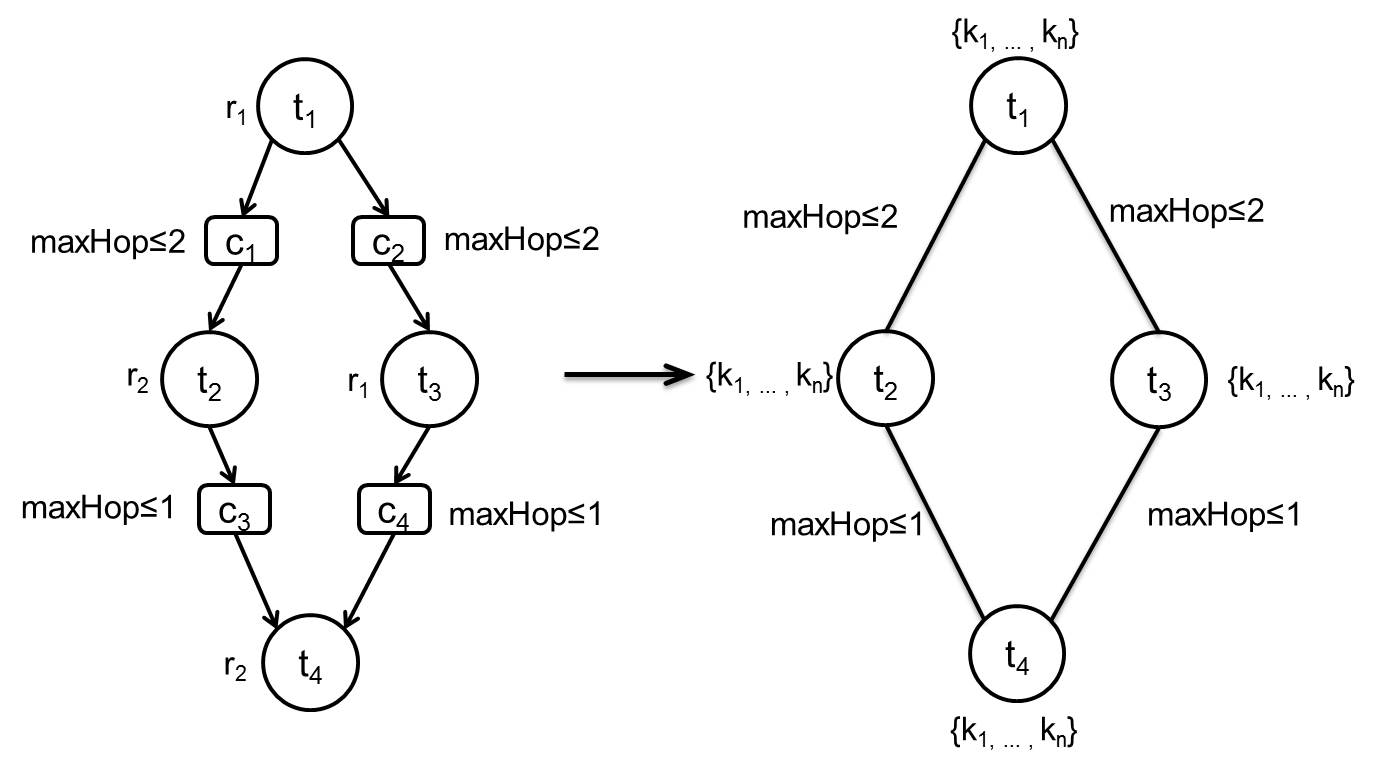
\includegraphics[width = 150mm]{bilder/taskConstraintgraph.jpg}
%  \caption{Transformation von einem Task- zu einem Constraintgraph}\label{fig:constraintgraph}
%\end{figure}

\section{Min-Conflicts-Embedder}
Die Min--Conflicts--Heuristik ist in der Praxis eine häufig eingesetzte Methode zum Lösen von CSPs. Es handelt sich nicht um ein systematisches Verfahren wie beim Backtracking, sondern um ein Stochastisches. Als Startpunkt wird eine zufällige Belegung der Veriablen erzeugt. Falls dies keine Lösung des CSPs ist, wovon auszugehen ist, wird eine konflikterzeugende Variable zufällig ausgewählt. Dieser wird ein Wert zugewiesen, der weniger Randbedingungen verletzt als der vorherige.\\ \\
Wie bei anderen stochastischen Methoden besteht auch hier die Gefahr, dass das System in einem lokalen Minimum terminiert. Falls das eintrifft, muss eine erneute zufällige Belegung der Variablen erzeugt werden und eine neue Runde beginnt. Eine Tabu-Liste kann dabei helfen, Belegungen, die zu einem lokalen Minimum geführt haben, nicht mehr zu wählen. Nach einer vorher festgelegten Anzahl von Runden beendet sich die Heuristik und das Scheitern der Einplanung wird ausgegeben. So kann es vorkommen, dass die Min--Conflicts-Heuristik keine konsistente Lösung findet, obwohl es eine im Constraint--System gibt.\\ \\
Oftmals wird die Heuristik verwendet, wenn sich das Constraint--System geringfügig verändert hat und für das vorherige System schon eine Lösung vorhanden ist. Aus diesem Grund wird der Algorithmus auch als "heuristisches Reparieren" \cite{cspsolvingRepairMethod} bezeichnet.\\ \\
